% Created by tikzDevice version 0.10.1 on 2016-12-09 07:37:51
% !TEX encoding = UTF-8 Unicode
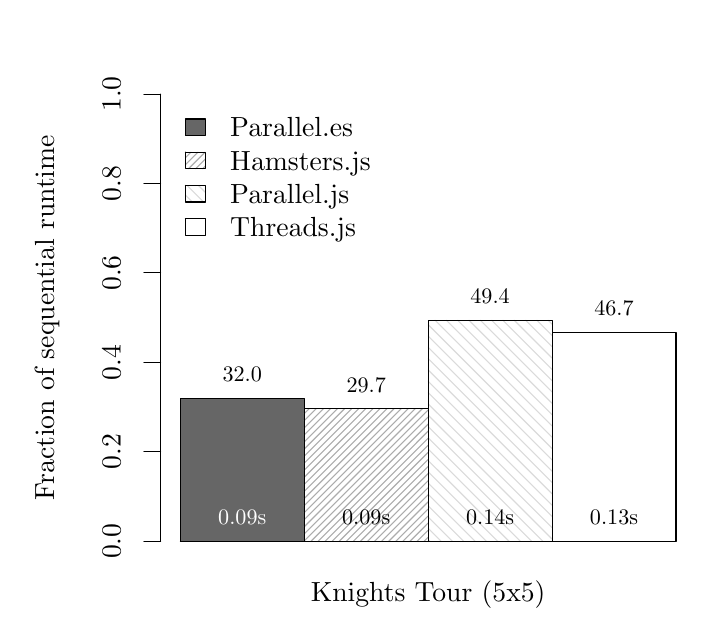
\begin{tikzpicture}[x=1pt,y=1pt]
\definecolor{fillColor}{RGB}{255,255,255}
\path[use as bounding box,fill=fillColor,fill opacity=0.00] (0,0) rectangle (241.43,209.58);
\begin{scope}
\path[clip] (  0.00,  0.00) rectangle (241.43,209.58);
\definecolor{fillColor}{gray}{0.40}

\path[fill=fillColor] ( 55.16, 24.00) --
	( 99.94, 24.00) --
	( 99.94, 75.63) --
	( 55.16, 75.63) --
	cycle;
\definecolor{drawColor}{RGB}{172,172,172}

\path[draw=drawColor,line width= 0.4pt,line join=round,line cap=round] ( 99.94, 70.11) -- (101.74, 71.91);

\path[draw=drawColor,line width= 0.4pt,line join=round,line cap=round] ( 99.94, 67.56) -- (104.29, 71.91);

\path[draw=drawColor,line width= 0.4pt,line join=round,line cap=round] ( 99.94, 65.00) -- (106.85, 71.91);

\path[draw=drawColor,line width= 0.4pt,line join=round,line cap=round] ( 99.94, 62.45) -- (109.40, 71.91);

\path[draw=drawColor,line width= 0.4pt,line join=round,line cap=round] ( 99.94, 59.89) -- (111.96, 71.91);

\path[draw=drawColor,line width= 0.4pt,line join=round,line cap=round] ( 99.94, 57.34) -- (114.51, 71.91);

\path[draw=drawColor,line width= 0.4pt,line join=round,line cap=round] ( 99.94, 54.78) -- (117.07, 71.91);

\path[draw=drawColor,line width= 0.4pt,line join=round,line cap=round] ( 99.94, 52.23) -- (119.62, 71.91);

\path[draw=drawColor,line width= 0.4pt,line join=round,line cap=round] ( 99.94, 49.67) -- (122.18, 71.91);

\path[draw=drawColor,line width= 0.4pt,line join=round,line cap=round] ( 99.94, 47.12) -- (124.74, 71.91);

\path[draw=drawColor,line width= 0.4pt,line join=round,line cap=round] ( 99.94, 44.56) -- (127.29, 71.91);

\path[draw=drawColor,line width= 0.4pt,line join=round,line cap=round] ( 99.94, 42.01) -- (129.85, 71.91);

\path[draw=drawColor,line width= 0.4pt,line join=round,line cap=round] ( 99.94, 39.45) -- (132.40, 71.91);

\path[draw=drawColor,line width= 0.4pt,line join=round,line cap=round] ( 99.94, 36.90) -- (134.96, 71.91);

\path[draw=drawColor,line width= 0.4pt,line join=round,line cap=round] ( 99.94, 34.34) -- (137.51, 71.91);

\path[draw=drawColor,line width= 0.4pt,line join=round,line cap=round] ( 99.94, 31.79) -- (140.07, 71.91);

\path[draw=drawColor,line width= 0.4pt,line join=round,line cap=round] ( 99.94, 29.23) -- (142.62, 71.91);

\path[draw=drawColor,line width= 0.4pt,line join=round,line cap=round] ( 99.94, 26.68) -- (144.71, 71.45);

\path[draw=drawColor,line width= 0.4pt,line join=round,line cap=round] ( 99.94, 24.12) -- (144.71, 68.90);

\path[draw=drawColor,line width= 0.4pt,line join=round,line cap=round] (102.37, 24.00) -- (144.71, 66.34);

\path[draw=drawColor,line width= 0.4pt,line join=round,line cap=round] (104.93, 24.00) -- (144.71, 63.79);

\path[draw=drawColor,line width= 0.4pt,line join=round,line cap=round] (107.48, 24.00) -- (144.71, 61.23);

\path[draw=drawColor,line width= 0.4pt,line join=round,line cap=round] (110.04, 24.00) -- (144.71, 58.68);

\path[draw=drawColor,line width= 0.4pt,line join=round,line cap=round] (112.59, 24.00) -- (144.71, 56.12);

\path[draw=drawColor,line width= 0.4pt,line join=round,line cap=round] (115.15, 24.00) -- (144.71, 53.57);

\path[draw=drawColor,line width= 0.4pt,line join=round,line cap=round] (117.70, 24.00) -- (144.71, 51.01);

\path[draw=drawColor,line width= 0.4pt,line join=round,line cap=round] (120.26, 24.00) -- (144.71, 48.45);

\path[draw=drawColor,line width= 0.4pt,line join=round,line cap=round] (122.81, 24.00) -- (144.71, 45.90);

\path[draw=drawColor,line width= 0.4pt,line join=round,line cap=round] (125.37, 24.00) -- (144.71, 43.34);

\path[draw=drawColor,line width= 0.4pt,line join=round,line cap=round] (127.92, 24.00) -- (144.71, 40.79);

\path[draw=drawColor,line width= 0.4pt,line join=round,line cap=round] (130.48, 24.00) -- (144.71, 38.23);

\path[draw=drawColor,line width= 0.4pt,line join=round,line cap=round] (133.04, 24.00) -- (144.71, 35.68);

\path[draw=drawColor,line width= 0.4pt,line join=round,line cap=round] (135.59, 24.00) -- (144.71, 33.12);

\path[draw=drawColor,line width= 0.4pt,line join=round,line cap=round] (138.15, 24.00) -- (144.71, 30.57);

\path[draw=drawColor,line width= 0.4pt,line join=round,line cap=round] (140.70, 24.00) -- (144.71, 28.01);

\path[draw=drawColor,line width= 0.4pt,line join=round,line cap=round] (143.26, 24.00) -- (144.71, 25.46);
\definecolor{drawColor}{RGB}{218,218,218}

\path[draw=drawColor,line width= 0.4pt,line join=round,line cap=round] (145.30, 24.00) -- (144.71, 24.59);

\path[draw=drawColor,line width= 0.4pt,line join=round,line cap=round] (149.39, 24.00) -- (144.71, 28.67);

\path[draw=drawColor,line width= 0.4pt,line join=round,line cap=round] (153.48, 24.00) -- (144.71, 32.76);

\path[draw=drawColor,line width= 0.4pt,line join=round,line cap=round] (157.56, 24.00) -- (144.71, 36.85);

\path[draw=drawColor,line width= 0.4pt,line join=round,line cap=round] (161.65, 24.00) -- (144.71, 40.94);

\path[draw=drawColor,line width= 0.4pt,line join=round,line cap=round] (165.74, 24.00) -- (144.71, 45.03);

\path[draw=drawColor,line width= 0.4pt,line join=round,line cap=round] (169.83, 24.00) -- (144.71, 49.11);

\path[draw=drawColor,line width= 0.4pt,line join=round,line cap=round] (173.92, 24.00) -- (144.71, 53.20);

\path[draw=drawColor,line width= 0.4pt,line join=round,line cap=round] (178.01, 24.00) -- (144.71, 57.29);

\path[draw=drawColor,line width= 0.4pt,line join=round,line cap=round] (182.09, 24.00) -- (144.71, 61.38);

\path[draw=drawColor,line width= 0.4pt,line join=round,line cap=round] (186.18, 24.00) -- (144.71, 65.47);

\path[draw=drawColor,line width= 0.4pt,line join=round,line cap=round] (189.49, 24.78) -- (144.71, 69.56);

\path[draw=drawColor,line width= 0.4pt,line join=round,line cap=round] (189.49, 28.87) -- (144.71, 73.64);

\path[draw=drawColor,line width= 0.4pt,line join=round,line cap=round] (189.49, 32.96) -- (144.71, 77.73);

\path[draw=drawColor,line width= 0.4pt,line join=round,line cap=round] (189.49, 37.05) -- (144.71, 81.82);

\path[draw=drawColor,line width= 0.4pt,line join=round,line cap=round] (189.49, 41.13) -- (144.71, 85.91);

\path[draw=drawColor,line width= 0.4pt,line join=round,line cap=round] (189.49, 45.22) -- (144.71, 90.00);

\path[draw=drawColor,line width= 0.4pt,line join=round,line cap=round] (189.49, 49.31) -- (144.71, 94.08);

\path[draw=drawColor,line width= 0.4pt,line join=round,line cap=round] (189.49, 53.40) -- (144.71, 98.17);

\path[draw=drawColor,line width= 0.4pt,line join=round,line cap=round] (189.49, 57.49) -- (144.71,102.26);

\path[draw=drawColor,line width= 0.4pt,line join=round,line cap=round] (189.49, 61.57) -- (147.23,103.83);

\path[draw=drawColor,line width= 0.4pt,line join=round,line cap=round] (189.49, 65.66) -- (151.32,103.83);

\path[draw=drawColor,line width= 0.4pt,line join=round,line cap=round] (189.49, 69.75) -- (155.41,103.83);

\path[draw=drawColor,line width= 0.4pt,line join=round,line cap=round] (189.49, 73.84) -- (159.50,103.83);

\path[draw=drawColor,line width= 0.4pt,line join=round,line cap=round] (189.49, 77.93) -- (163.59,103.83);

\path[draw=drawColor,line width= 0.4pt,line join=round,line cap=round] (189.49, 82.02) -- (167.67,103.83);

\path[draw=drawColor,line width= 0.4pt,line join=round,line cap=round] (189.49, 86.10) -- (171.76,103.83);

\path[draw=drawColor,line width= 0.4pt,line join=round,line cap=round] (189.49, 90.19) -- (175.85,103.83);

\path[draw=drawColor,line width= 0.4pt,line join=round,line cap=round] (189.49, 94.28) -- (179.94,103.83);

\path[draw=drawColor,line width= 0.4pt,line join=round,line cap=round] (189.49, 98.37) -- (184.03,103.83);

\path[draw=drawColor,line width= 0.4pt,line join=round,line cap=round] (189.49,102.46) -- (188.12,103.83);
\definecolor{drawColor}{RGB}{0,0,0}

\path[draw=drawColor,line width= 0.4pt,line join=round,line cap=round] ( 55.16, 24.00) --
	( 99.94, 24.00) --
	( 99.94, 75.63) --
	( 55.16, 75.63) --
	( 55.16, 24.00);

\path[draw=drawColor,line width= 0.4pt,line join=round,line cap=round] ( 99.94, 24.00) --
	(144.71, 24.00) --
	(144.71, 71.91) --
	( 99.94, 71.91) --
	( 99.94, 24.00);

\path[draw=drawColor,line width= 0.4pt,line join=round,line cap=round] (144.71, 24.00) --
	(189.49, 24.00) --
	(189.49,103.83) --
	(144.71,103.83) --
	(144.71, 24.00);

\path[draw=drawColor,line width= 0.4pt,line join=round,line cap=round] (189.49, 24.00) --
	(234.26, 24.00) --
	(234.26, 99.46) --
	(189.49, 99.46) --
	(189.49, 24.00);
\end{scope}
\begin{scope}
\path[clip] (  0.00,  0.00) rectangle (241.43,209.58);
\definecolor{drawColor}{RGB}{0,0,0}

\node[text=drawColor,anchor=base,inner sep=0pt, outer sep=0pt, scale=  1.00] at (144.71,  2.40) {Knights Tour (5x5)};
\end{scope}
\begin{scope}
\path[clip] (  0.00,  0.00) rectangle (241.43,209.58);
\definecolor{drawColor}{RGB}{0,0,0}

\node[text=drawColor,rotate= 90.00,anchor=base,inner sep=0pt, outer sep=0pt, scale=  1.00] at (  9.60,104.79) {Fraction of sequential runtime};
\end{scope}
\begin{scope}
\path[clip] (  0.00,  0.00) rectangle (241.43,209.58);
\definecolor{drawColor}{RGB}{0,0,0}

\path[draw=drawColor,line width= 0.4pt,line join=round,line cap=round] ( 48.00, 24.00) -- ( 48.00,185.58);

\path[draw=drawColor,line width= 0.4pt,line join=round,line cap=round] ( 48.00, 24.00) -- ( 42.00, 24.00);

\path[draw=drawColor,line width= 0.4pt,line join=round,line cap=round] ( 48.00, 56.32) -- ( 42.00, 56.32);

\path[draw=drawColor,line width= 0.4pt,line join=round,line cap=round] ( 48.00, 88.63) -- ( 42.00, 88.63);

\path[draw=drawColor,line width= 0.4pt,line join=round,line cap=round] ( 48.00,120.95) -- ( 42.00,120.95);

\path[draw=drawColor,line width= 0.4pt,line join=round,line cap=round] ( 48.00,153.27) -- ( 42.00,153.27);

\path[draw=drawColor,line width= 0.4pt,line join=round,line cap=round] ( 48.00,185.58) -- ( 42.00,185.58);

\node[text=drawColor,rotate= 90.00,anchor=base,inner sep=0pt, outer sep=0pt, scale=  1.00] at ( 33.60, 24.00) {0.0};

\node[text=drawColor,rotate= 90.00,anchor=base,inner sep=0pt, outer sep=0pt, scale=  1.00] at ( 33.60, 56.32) {0.2};

\node[text=drawColor,rotate= 90.00,anchor=base,inner sep=0pt, outer sep=0pt, scale=  1.00] at ( 33.60, 88.63) {0.4};

\node[text=drawColor,rotate= 90.00,anchor=base,inner sep=0pt, outer sep=0pt, scale=  1.00] at ( 33.60,120.95) {0.6};

\node[text=drawColor,rotate= 90.00,anchor=base,inner sep=0pt, outer sep=0pt, scale=  1.00] at ( 33.60,153.27) {0.8};

\node[text=drawColor,rotate= 90.00,anchor=base,inner sep=0pt, outer sep=0pt, scale=  1.00] at ( 33.60,185.58) {1.0};
\end{scope}
\begin{scope}
\path[clip] ( 48.00, 24.00) rectangle (241.43,185.58);
\definecolor{fillColor}{gray}{0.40}

\path[fill=fillColor] ( 57.00,176.58) --
	( 64.20,176.58) --
	( 64.20,170.58) --
	( 57.00,170.58) --
	cycle;
\definecolor{drawColor}{RGB}{172,172,172}

\path[draw=drawColor,line width= 0.4pt,line join=round,line cap=round] ( 57.00,162.60) -- ( 58.99,164.58);

\path[draw=drawColor,line width= 0.4pt,line join=round,line cap=round] ( 57.00,160.04) -- ( 61.54,164.58);

\path[draw=drawColor,line width= 0.4pt,line join=round,line cap=round] ( 58.10,158.58) -- ( 64.10,164.58);

\path[draw=drawColor,line width= 0.4pt,line join=round,line cap=round] ( 60.65,158.58) -- ( 64.20,162.13);

\path[draw=drawColor,line width= 0.4pt,line join=round,line cap=round] ( 63.21,158.58) -- ( 64.20,159.58);
\definecolor{drawColor}{RGB}{218,218,218}

\path[draw=drawColor,line width= 0.4pt,line join=round,line cap=round] ( 59.51,146.58) -- ( 57.00,149.09);

\path[draw=drawColor,line width= 0.4pt,line join=round,line cap=round] ( 63.60,146.58) -- ( 57.60,152.58);

\path[draw=drawColor,line width= 0.4pt,line join=round,line cap=round] ( 64.20,150.07) -- ( 61.69,152.58);
\definecolor{drawColor}{RGB}{0,0,0}

\path[draw=drawColor,line width= 0.4pt,line join=round,line cap=round] ( 57.00,176.58) --
	( 64.20,176.58) --
	( 64.20,170.58) --
	( 57.00,170.58) --
	( 57.00,176.58);

\path[draw=drawColor,line width= 0.4pt,line join=round,line cap=round] ( 57.00,164.58) --
	( 64.20,164.58) --
	( 64.20,158.58) --
	( 57.00,158.58) --
	( 57.00,164.58);

\path[draw=drawColor,line width= 0.4pt,line join=round,line cap=round] ( 57.00,152.58) --
	( 64.20,152.58) --
	( 64.20,146.58) --
	( 57.00,146.58) --
	( 57.00,152.58);

\path[draw=drawColor,line width= 0.4pt,line join=round,line cap=round] ( 57.00,140.58) --
	( 64.20,140.58) --
	( 64.20,134.58) --
	( 57.00,134.58) --
	( 57.00,140.58);

\node[text=drawColor,anchor=base west,inner sep=0pt, outer sep=0pt, scale=  1.00] at ( 73.20,170.14) {Parallel.es};

\node[text=drawColor,anchor=base west,inner sep=0pt, outer sep=0pt, scale=  1.00] at ( 73.20,158.14) {Hamsters.js};

\node[text=drawColor,anchor=base west,inner sep=0pt, outer sep=0pt, scale=  1.00] at ( 73.20,146.14) {Parallel.js};

\node[text=drawColor,anchor=base west,inner sep=0pt, outer sep=0pt, scale=  1.00] at ( 73.20,134.14) {Threads.js};

\node[text=drawColor,anchor=base,inner sep=0pt, outer sep=0pt, scale=  0.80] at ( 77.55, 81.63) {32.0};

\node[text=drawColor,anchor=base,inner sep=0pt, outer sep=0pt, scale=  0.80] at (122.33, 77.91) {29.7};

\node[text=drawColor,anchor=base,inner sep=0pt, outer sep=0pt, scale=  0.80] at (167.10,109.83) {49.4};

\node[text=drawColor,anchor=base,inner sep=0pt, outer sep=0pt, scale=  0.80] at (211.88,105.46) {46.7};
\definecolor{drawColor}{RGB}{255,255,255}

\node[text=drawColor,anchor=base,inner sep=0pt, outer sep=0pt, scale=  0.80] at ( 77.55, 30.00) {0.09s};
\definecolor{drawColor}{RGB}{0,0,0}

\node[text=drawColor,anchor=base,inner sep=0pt, outer sep=0pt, scale=  0.80] at (122.33, 30.00) {0.09s};

\node[text=drawColor,anchor=base,inner sep=0pt, outer sep=0pt, scale=  0.80] at (167.10, 30.00) {0.14s};

\node[text=drawColor,anchor=base,inner sep=0pt, outer sep=0pt, scale=  0.80] at (211.88, 30.00) {0.13s};
\end{scope}
\end{tikzpicture}
